\documentclass[border=0pt]{standalone}

\usepackage{enumitem}

\usepackage[sc]{mathpazo}
\usepackage{tikz}
\linespread{1.05}

\newcommand\bluebullet{%
  \tikz[baseline=0ex]\fill[blue!75!black]
    (0,0)--(0.18,0.09)--(0,0.18)--cycle;}


\usepackage[table]{xcolor}
\definecolor{petrol}{RGB}{117,208,98}


\usepackage{tikz}
\usetikzlibrary{calc}


\usepackage{ragged2e}

\begin{document}
\small

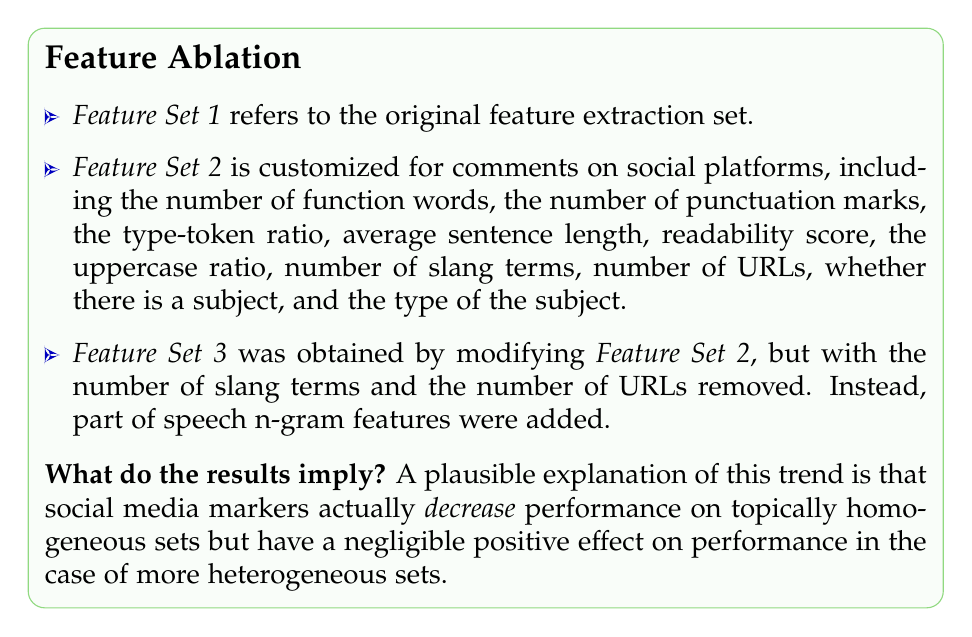
\begin{tikzpicture}
\node[
  draw=petrol!80,              
  fill=petrol!4,              
  rounded corners=6pt,
  minimum width=0.1\linewidth, 
  inner sep=6pt,               
  text width=0.97\linewidth-16pt, 
  font=\normalsize,
  align=justify                
] (cap) {%
  \noindent {\large\textbf{Feature Ablation}}
\begin{itemize}[label=\bluebullet,left=0em,itemsep=3pt]
  \item \textit{Feature Set 1} refers to the original feature extraction set. 
  \item \textit{Feature Set 2} is customized for comments on social platforms, including the number of function words, the number of punctuation marks, the type-token ratio, average sentence length, readability score, the uppercase ratio, number of slang terms, number of URLs, whether there is a subject, and the type of the subject.
  \item \textit{Feature Set 3} was obtained by modifying \textit{Feature Set 2}, but with the number of slang terms and the number of URLs removed. Instead, part of speech n-gram features were added.
\end{itemize}
\noindent {\normalsize\textbf{What do the results imply?} A plausible explanation of this trend is that social media markers actually \textit{decrease} performance on topically homogeneous sets but have a negligible positive effect on performance in the case of more heterogeneous sets.}
  };
\end{tikzpicture}

\end{document}